%\title{Creating an index with the makeidx package}
% Example from http://www.dickimaw-books.com/latex/thesis/html/makeidx.html

\documentclass[12pt,oneside]{scrbook} 

\usepackage{makeidx} 
\usepackage{minted}
\usepackage[french]{babel}
\usepackage{graphicx}
\selectlanguage{french}
\usepackage[T1]{fontenc}
\usepackage[utf8]{inputenc}
\usepackage{xcolor}
\definecolor{bg}{rgb}{0.95,0.95,0.95}
\definecolor{bg_js}{rgb}{0.95,0.55,0.55}
\newminted{typescript}{javascript,bgcolor=bg}

\makeindex 

\title{Typescript/NodeJS} 
\author{Me}
\date{\today}

\begin{document} 
\maketitle 
\tableofcontents


%%%%%%%%%%%%%%NPM/Node
\chapter{NPM/Node}
\section{Commandes}
\begin{itemize}
\item Initialisation d'un projet\\
La commande \textit{init} permet de créer un projet .json vide
\item Installation d'un module\\
Dans un projet existant, on peut rajouter un module et en même temps la dépendance:
\begin{minted}[bgcolor=bg]{shell}
npm install "module" -D
\end{minted}
\item Ajouter automatiquement ce module en dépendance de développement
\begin{minted}[bgcolor=bg]{shell}
npm install "module" -D
\end{minted}
\item Ajouter automatiquement ce module en dépendance de livraison
\begin{minted}[bgcolor=bg]{shell}
npm install "module" --save
\end{minted}
\item Lancer un script\\
Dans la liste des scripts du fichier .json, il peut être possible d'en lancer un:
\begin{minted}[bgcolor=bg]{shell}
npm run es6
\end{minted}
Dans cet exemple:
\begin{minted}[bgcolor=bg]{shell}
"scripts": {
    "es6": "./node_modules/.bin/http-server -c-1 ."
  }
\end{minted}
\item Débogage dans Chrome\\
On peut lancer un debogage d'un fichier JS depuis Node. Celui-ci lance un browker permettant par la suite de deboguer depuis les devtools de Chrome gràce au lien renvoyé par cette commande:
\begin{minted}[bgcolor=bg]{shell}
node --debug-brk=35220 --inspect samples\learning-types.js
\end{minted}
\end{itemize}

\section{V8}
Le moteur V8 transforme le langage JS en langage machine:

Javascript --> C/C++ --> Assembleur --> Langage machine

Node est codé en C++ car V8 est codé en C++.

\section{CommonJS}
C'est un ensemble de standards définissant comment structures les modules NodeJS

\section{First Class Functions}
Ce que l'on peut faire avec les types, on peut le faire avec les first Class Functions.
\begin{minted}[bgcolor=bg]{javascript}
function greet()
{
    console.log("coucou");
}
greet();
//functions are first-class
function logGreeting(fn)
{
    fn();
}
logGreeting(greet);
//function expression
var greetMe = function()
{
    console.log("coucou");
}
greetMe();
//it's first class
logGreeting(greetMe);
//use a function expression on the fly
logGreeting(function()
    {
        console.log('coucou3');
        
    }
);
\end{minted}


\section{Modules}
Afin d'accéder aux fonctionnalités d'un autre fichier, on utilise \textit{require}.
\begin{minted}[bgcolor=bg]{javascript}
//fichier app.js
require("./greet.js");

//fichier greet.js
console.log('salut');
\end{minted}
Ceci fonctionne. Cependant le code suivant ne fonctionne pas:
\begin{minted}[bgcolor=bg]{javascript}
//fichier app.js
require("./greet.js");
greet();

//fichier greet.js
function greet() {
	console.log('salut');
}
\end{minted}
Ceci parce que la variable \textit{greet} n'est pas accéssible depuis un autre fichier. Pour pouvoir le faire, il faut la rendre accéssible avec la notion d'exportation:
\begin{minted}[bgcolor=bg]{javascript}
//fichier app.js
var greet = require("./greet.js");
greet();

//fichier greet.js
function greet()
{
    console.log('salut');
}
module.exports = greet;
\end{minted}

%%%%%%%%%%%%Retour sur ES6
\chapter{Retour sur ES6} 
Avant de parler de TypeScript, Un petit aperçu de certaines fonctionnalités de ES6
\section{Concaténation de chaîne avec `}
\index{symbole `}
Permet de concaténer des chaînes, au lieu de faire:

\begin{minted}[bgcolor=bg]{javascript}
unevar='mon texte '+machaine;
\end{minted}
On peut écrire:
\begin{minted}[bgcolor=bg]{javascript}
`mon texte ${machaine}`;
\end{minted}

\section{Object destructuring}
Lors du passage d'un objet en paramètre, on peut préciser directement les propriétés que l'on veut utiliser et ainsi faire un raccourci sur les variables interne à la fonction:\\
Avant:
\begin{minted}[bgcolor=bg]{javascript}
function buildPersonData(personData)
{
    return personData.firstName + ' ' +
    personData.lastName + ' ' +
    personData.address;
}
\end{minted}
Après:
\begin{minted}[bgcolor=bg]{javascript}
function buildPersonData({firstName, lastName, address})
{
    return `$firstName  $lastName $address`;
}
\end{minted}
\section{Shorthand Object Creation}
Quand une propriété a le même nom qu'une variable, on peut faire un raccourci:\\
Avant:
\begin{minted}[bgcolor=bg]{javascript}
const 
    firstName='Kobe',
    lastName='Bryant',
    address='staples Center'

const personData = {
    firstName:firstName, //répétition de nom
    lastName:lastName,   //répétition de nom
    address:address      //répétition de nom
};
\end{minted}
Après:
\begin{minted}[bgcolor=bg]{javascript}
const 
    firstName='Kobe',
    lastName='Bryant',
    address='staples Center'

const personData = {
    firstName,
    lastName,
    address
};
\end{minted}
Stuff about eigenvectors\index{eigenvector} and 
eigenvalues\index{eigenvalue}. 

\begin{minted}[bgcolor=bg]{c}
int main() {
  printf("hello, world");
  return 0;
}
\end{minted}
\section{Notion d'objects}
\begin{itemize}
\item \textbf{Définition}: D'un point de vue Javascript, un objet est un ensemble de paire Clé/Valeur.
\item \textbf{Objet littéral}: Possibilité de créer un objet directement depuis un ensemble de clé/valeur séparées par des virgules et encadrées par des accolades.
\begin{minted}[bgcolor=bg]{javascript}
var obj = 
{
    name:"Pouet",
    adresse:
    {
        rue:"23 rue du truc",
        cp: 59000
    }
}
console.log(obj);
\end{minted}
La sortie sera:
\begin{minted}[bgcolor=bg]{javascript}
{ name: 'Pouet', adresse: { rue: '23 rue du truc', cp: 59000 } }
\end{minted}
On peut y déclarer des fonctions:
\begin{minted}[bgcolor=bg]{javascript}
var obj = 
{
    name:"Pouet",
    adresse:
    {
        rue:"23 rue du truc",
        cp: 59000
    },
    greet: function() {
        console.log('coucou');
    }
}
console.log(obj);
obj.greet();
\end{minted}
\item \textbf{Accès}: Les accès aux propriétés/fonctions peuvent se faire de différentes manière:
\begin{minted}[bgcolor=bg]{javascript}

obj.greet();
//ou
obj['greet']();
\end{minted}
\end{itemize}

\section{function Expressions (IIFEs/Immediatly Invoked Function Expression)}
Il s'agit d'une fonction directement présente dans une expression. Elle se trouve entre parenthèse.

\begin{minted}[bgcolor=bg]{javascript}
(function (lastname) {

    var firstname = 'John';
    console.log(firstname);
    console.log(lastname);
	
}('Doe'));
\end{minted}


%%%%%chaine des prototypes
\section{Simulation héritage avec la méthode ES6}
Il est possible de faire des simulations d'héritage en javascript ES6 avec les prototypes.

\begin{minted}[bgcolor=bg]{javascript}
var person  ={
    firstname:'',
    lastname:'Doe',
    greet:function() {
        return this.firstname+' '+this.lastname;
    }
}
\end{minted}
Ce premier prototype sert de "classe de base" pour notre futur "objet". On utilise alors \textit{Object.create} pour effectuer l'association des prototype de notre "objet" avec celui de la "classe".
\begin{minted}[bgcolor=bg]{javascript}
var john = Object.create(person);
john.firstname = 'John';
john.lastname  = 'Doe\'s';
\end{minted}
Les attributs \textit{firstname} et \textit{lastname} sont surchargés.
\begin{minted}[bgcolor=bg]{javascript}
console.log(john.greet());
\end{minted}
Avec cette commande on invoque la commande \textit{greet} qui est en fait la commande \textit{greet} de la "classe". Alors que faire \textit{console.log(john.firstname)} invoque en réalité la propriété \textit{lastname} de l'objet John, sans passer donc par la prototype.

On peut empiler la création d'objet et le chaînage des prototypes:
\begin{minted}[bgcolor=bg]{javascript}
var subJohn = Object.create(john);
subJohn.firstname = 'SubJohn';
console.log(subJohn.greet());
\end{minted}
Ici, subJohn \textit{hérite} des propriété de john, on ajoute en réalité un nouveau maillon dans le chaînage des prototypes. Utiliser la propriété \textit{firstname} de subJohn ne passe par aucun prototype puisqu'il a été surchargé. En revanche, appeler \textit{greet} est en fait le prototype du prototype de john.
On uilise pour se faire la chaine des prototypes comme expliqué dans le shéma suivant:

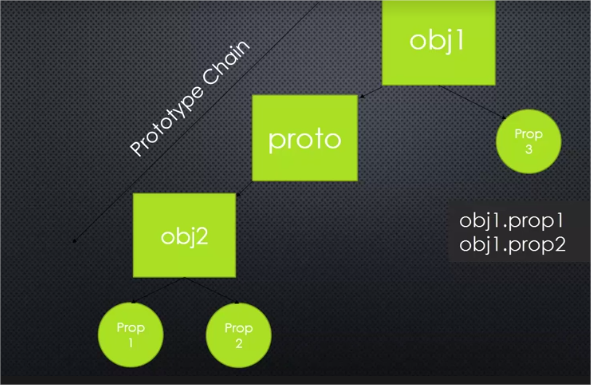
\includegraphics{chaine_proto.png}
Nous voyons dans ce schéma que \textit{obj1} a pour prototype \textit{obj2}. Ce dernier possède les propriétés \textit{prop1} et \textit{prop2}, alors que \textit{obj1} n'a que \textit{prop3}. Et pourtant écrire les commandes suivantes est correct:
\begin{minted}[bgcolor=bg]{javascript}
//correct, le chaînage des prototypes remonte à obj2
console.log(obj1.prop1);
//correct aussi, le chaîne remonte à nouveau à obj2
console.log(obj1.prop2);
//toujours correct, sauf que le chaîne s'arrête à obj1
console.log(obj1.prop3);
\end{minted}
\section{Simulation héritage avec la méthode NodeJS}
Une autre méthode consiste à utiliser la méthode \textit{inherits} située dans les utilitaires de NodeJS. Contrairement à un héritage dans un langage Objet où l'on créé la classe directement en spécifiant sa classe de base, ici on créé l'objet, et on indique de quoi il \textit{hérite}.
\begin{minted}[bgcolor=bg]{javascript}
var EventEmitter = require('events');
var util = require('util');
//Création de l'objet de base
function Greetr() {
    this.greeting = 'Hello world';
}
//Héritage de events, représenté par la variable EventEmitter
util.inherits(Greetr, EventEmitter);
//création d'une méthode propre à Greetr MAIS
//dans laquelle maintenant on peut faire appel
//a une méthode de EventEmitter
Greetr.prototype.greet = function()
{
    console.log(this.greeting);
    //méthode "heritée"
    this.emit('greet');
}
//et enfin l'objet qui instancie le tout
greeter1 = new Greetr();
greeter1.on('greet', function() {
    console.log('on m\'a salué');
});
greeter1.greet();
\end{minted}
Le schéma suivant explique ce qu'il s'est passé:

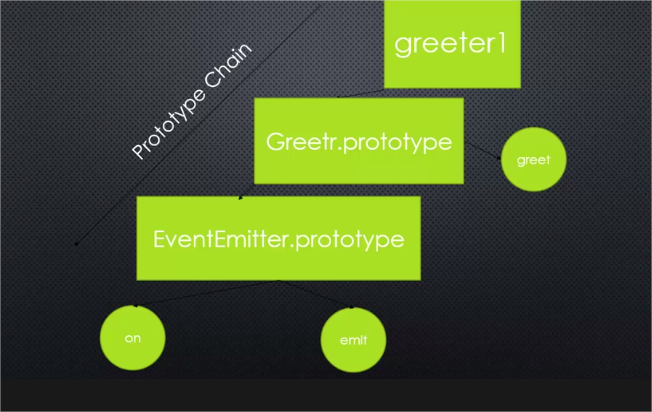
\includegraphics{util_inherits.png}

\chapter{TypeScript}
On entre dans le vif du sujet avec TypeScript
\section{Présentation}
\begin{itemize}
\item Avoir la version
\begin{minted}[bgcolor=bg]{bash}
./node_modules/.bin/tsc -version
\end{minted}
\item Configuration dans Visual Code\\
Il faut créer un nouveau fichier \textit{tsconfig.json}:
\begin{minted}[bgcolor=bg]{json}
{
    "compilerOptions":
    {
        "target":"es5",
        "module":"commonjs",
        "sourceMap":true
    }
}
\end{minted}
\item Compiler du ts sous Visual Code\\
Lancer la commande \textit{CTRL+SHIFT+b} pour lancer une compilation. Visual Code dira qu'il n'y a pas de configuration de build associée au projet, alors il en proposera de choisir le langage. Il faut choisir \textit{typescript:tsconfig.json}. Un fichier \textit{tasks.json} est crée.
\end{itemize}


%%%%%%    Portée des var/let
\section{Portée des var/let}
La déclaration d'une variable avec \textit{var} retire la portée réelle de cette variable et est donc source de problème.
\begin{minted}[bgcolor=bg]{javascript}
if(1)
{
    var mavaleur = 12;
}
mavaleur = 12; //!!!toujours à portée alors que théoriquement non!!!!
\end{minted}
Avec la commande \textit{let}
\begin{minted}[bgcolor=bg]{javascript}
if(1)
{
    let mavaleur = 12;
}
mavaleur = 12; //!!!erreur: hors de portée, ce qui est plus clair!!!!
\end{minted}


%%%%%%    TYPE
\section{Les types}
\noindent
\textbf{Les types primitifs}:
\begin{minted}[bgcolor=bg]{typescript}
const message:string = 'Hello Wolrd!';
const counter:number= 0;
\end{minted}
\noindent
\textbf{Les définitions d'objet}:

\begin{minted}[bgcolor=bg]{typescript}
let person = {
    firstName:'moi',
    lastName:'poi'
};
//impossible, pas de propriété 'address' définie
person.address = '';
\end{minted}
Autre façon de déclarer un objet:

\begin{minted}[bgcolor=bg]{typescript}
let person:{firstName:string, lastName:string} = {
    firstName:'moi',
    lastName:'poi'
};
\end{minted}
Maintenant avec cette méthode, il est possible de rendre un objet plus souple:
\begin{minted}[bgcolor=bg]{typescript}
let person:any = {
    firstName:'moi',
    lastName:'poi'
};
//possible, l'objet accepte tout
person.address = '';
\end{minted}
\noindent
\textbf{Les définitions de type}:

\begin{minted}[bgcolor=bg]{typescript}
type HasName = {firstName:string, lastName:string};
let person:any = {
    firstName:'moi',
    lastName:'poi'
};
\end{minted}
Possibilité de rendre un champ optionnel:

\begin{minted}[bgcolor=bg]{typescript}
type HasName = {
    //ce champ est optionnel
    firstName?:string, 
    lastName:string
};
//le champ 'firstName' n'est pas renseigné
let person:HasName = {
    lastName:'poi'
};
\end{minted}
Composition de type:
\begin{minted}[bgcolor=bg]{typescript}
type HasName = {
    firstName?:string, 
    lastName:string
};
type HasAddress = {
    streetName:string;
};
type Person =
{
    name:HasName,
    address:HasAddress
};
let person:Person = {
    name:{
        lastName:'poi'
    },
    address:{
        streetName:'une adresse'
    }
};
person.address.streetName = '';
\end{minted}
Définition de type pour une fonction:
\begin{minted}[bgcolor=bg]{typescript}
//définition du type, fonction avec un seul 
//paramètre qui renvoie un string
type MessageCreator = (name:string)=> string;
function createHelloMessage(name:string, extra?:number):string
{
    return `my name is ${name} et ${extra}`;
}
//cette affectation est possible car 'extra' est un paramètre facultatif
//pour la fonction createHelloMessage
const creator:MessageCreator = createHelloMessage;
//creator est devenu un pointeur sur fonction qu'il est possible d'appeler
const messageHello = creator('Bill');
console.log(messageHello);
\end{minted}




%%%%%%    Modules
\section{Modules}
Afin d'avoir la possibilité d'utiliser une variable/classe/constante/fonction dans un autre fichier, il faut les déclarer avec la commande \textit{export}:
\begin{minted}[bgcolor=bg]{typescript}
//export d'une fonction
export function buildPersonData (
    {firstName, lastName}, ...address) {
    return `${firstName} ${lastName} ${address}`;
}
//pour une constante
export const DEMO = 'demo';
\end{minted}
Ensuite, pour importer, il faut pouvoir préciser ce que l'on veut importer avec la commande \textit{import}:
\begin{minted}[bgcolor=bg]{typescript}
import {buildPersonData, DEMO} from "./buildPersonData";
\end{minted}
Le code généré est le suivant:
\begin{minted}[bgcolor=bg_js]{javascript}
"use strict";
Object.defineProperty(exports, "__esModule", { value: true });
var buildPersonData_1 = require("./buildPersonData");
/* ... */
\end{minted}
\textbf{Problème!!}\\
Dans les génération de code, \textit{exports} et \textit{require} n'existent pas. Cela est dû au fait que Typescript compile en tenant compte d'un module externe \textit{commonjs}, non inclu dans les navigateurs.

Il faut implémenter un module externe afin d'être capable d'utiliser les commandes \textit{require} et \textit{export} directement dans le fichier HTML:
\begin{minted}[bgcolor=bg]{html}
<script src="https://npmcdn.com/systemjs@0.19.27/dist/system.src.js">
</script>

<script>
//System.config afin d'éviter une erreur lors de la recherche 
//d'un fichier sans le .js
//Par defaut, import recherche un fichier sans extension,
//il faut donc préciser 'defaultJSExtensions' à true afin
//qu'il recherche '.js'
System.config({
defaultJSExtensions:true
});

System.import('/samples/hello-world');

</script>
\end{minted}
\begin{listing}[ht]
\begin{minted}[bgcolor=bg]{html}
<script src="https://npmcdn.com/systemjs@0.19.27/dist/system.src.js">
</script>

<script>
//System.config afin d'éviter une erreur lors de la recherche 
//d'un fichier sans le .js
//Par defaut, import recherche un fichier sans extension,
//il faut donc préciser 'defaultJSExtensions' à true afin
//qu'il recherche '.js'
System.config({
defaultJSExtensions:true
});

System.import('/samples/hello-world');

</script>
\end{minted}
\caption{Example from external file}
\label{listing:0}
\end{listing}



%%%%%%%%% ARROW
\section{Arrow =>}
Un arrow permet ede définir une fonction sans créer un nouveau scope pour la définition des variables:
\begin{listing}[ht]
\begin{minted}[bgcolor=bg]{typescript}
function mafonc(name:string)
{
/*...*/
}
\end{minted}
\caption{Avec scope, sans arrow}
\label{listing:0}
\end{listing}
\begin{listing}[ht]
\begin{minted}[bgcolor=bg]{typescript}
const maArrowFonc = (name:string) =>
{
/*...*/
}
\end{minted}
\caption{Sans scope, avec arrow}
\label{listing:0}
\end{listing}


%%%%%%Enum
\section{Déclarion d'un Enum}
La définition d'un Enum se fait simplement
\begin{minted}[bgcolor=bg]{typescript}
//on peut forcer l'un des champs à une valeur
enum MyPosition
{
  Un=5,
  Deux,
  Trois
}
//utilisation
console.log(MyPosition.Trois);
console.log(MyPosition["Trois"]);
\end{minted}


%%%%%%Decorators
\section{Decorators}
Un decorators permet de contrôler une méthode où est appliqué le décorateur
\begin{itemize}
\item Ajout d'un decorator\\
\begin{minted}[bgcolor=bg]{typescript}
class Database {
@LogArguments(LoggingLevel.DEBUG)
    saveData(data:any) {
        console.log('save data in the database ...');
    }
}
//définition du decorators
function LogArguments(level: LoggingLevel) {
    return (target: any, propertyKey: string, 
    descriptor: PropertyDescriptor) => {
        if (level >= loggingLevel) {
            console.log(`>>> ${target.arguments}`);
        }
        return target;
    }
}
\end{minted}

\item Définition des propriétés du decorator\\
--- \textbf{target}: il s'agit de la cible visée par le decorator. Dans le cas précédent, il s'agit de la classe  \textit{Database}

--- \textbf{propertyKey}: Dans le cas précédent il s'agit de la methode \textit{saveData}.

--- \textbf{descriptor}: Il s'agit d'une structure contenant des propriétés sur l'objet visé par le decorator. Par exemple \textit{value} représente dans le cas précédent la fonction elle-même, il est alors possible de la redéfinir.
\begin{minted}[bgcolor=bg]{typescript}
descriptor {
    value:[Function],
    writable:true,
    enumerable:true,
    configurable:true
}
\end{minted}

\item Exemple: Remplacement d'une fonction
\begin{minted}[bgcolor=bg]{typescript}
function LogArguments(level: LoggingLevel) {
    return (target: any, propertyKey: string, 
    descriptor: PropertyDescriptor) => {
        descriptor.value = () =>
        {
            console.log('new function');
        }
    }
}
\end{minted}
Dans cet exemple, l'appel de la fonction \textit{saveData} aura pour effet d'afficher \textit{'new function'} au lieu de \textit{'save data in the database ...'}. L'ancienne fonction est remplacée.
\item Exemple: Amélioration d'une fonction
Il est rare de vouloir remplacer une fonction, au lieu de ça, on va l'améliorer.
\begin{minted}[bgcolor=bg]{typescript}
function LogArguments(level: LoggingLevel) {
    return (target: any, propertyKey: string, 
    descriptor: PropertyDescriptor) => {
        //sauvegarde de la fonction originale
        const originalFunction = descriptor.value;
        descriptor.value = () =>
        {
            console.log('new function');
            //appel de la fonction originale
            originalFunction();
        }
    }
}
\end{minted}
Cette fois, la nouvelle fonction est appelée, et celle-ci, grace à la variable \textit{originalFunction}, appelle la fonction originale.
\end{itemize}


\backmatter 

\printindex 

\end{document} 